\documentclass[11pt]{report}
\usepackage[english]{babel}
\usepackage[T1]{fontenc}
\usepackage[utf8]{inputenc}
\usepackage{graphicx}
\usepackage{fancyhdr}
\usepackage{vmargin}									
\usepackage{hyperref}
\usepackage{subfig}
\usepackage{booktabs}
\usepackage{longtable}
\setmarginsrb{2.5 cm}{2.5 cm}{2.5 cm}{2.5 cm}{1 cm}{1.5 cm}{1 cm}{1.5 cm}
\graphicspath{{images/}}

\usepackage[dvipsnames]{xcolor}
\usepackage{listings}
\lstdefinelanguage{json}{
	basicstyle=\scriptsize\ttfamily,
	string=[s]{"}{"},
	stringstyle=\color{blue},
	comment=[l]{:},
	commentstyle=\color{black},
}

\lstdefinelanguage{JavaScript}{
	basicstyle=\scriptsize\ttfamily,
	keywords={typeof, new, true, false, catch, function, return, null, catch, switch, var, if, in, while, do, else, case, break, const, let},
	keywordstyle=\color{blue}\bfseries,
	ndkeywords={class, export, boolean, throw, implements, import, this},
	ndkeywordstyle=\color{darkgray}\bfseries,
	identifierstyle=\color{black},
	sensitive=false,
	comment=[l]{//},
	morecomment=[s]{/*}{*/},
	commentstyle=\color{ForestGreen}\ttfamily,
	stringstyle=\color{red}\ttfamily,
	morestring=[b]',
	morestring=[b]"
}

\title{HKRecruitment Project Specifications}				        % Title
%\author{Riccardo Zaccone}						            % Author
\author{Riccardo Zaccone \\ Arianna Ravera}   % Authors
\date{\today}										    % Date
%\date{08 novembre 2020}								    % Date

\makeatletter
\let\thetitle\@title
\let\theauthor\@author
\let\thedate\@date
\makeatother

\hypersetup{
	pdftitle={\thetitle},
	pdfauthor={\theauthor},
	pdfsubject={},
	pdfkeywords={},
	hidelinks}

\pagestyle{fancy}
\fancyhf{}
\lhead{\thetitle}
\cfoot{\thepage}

\begin{document}

%%%%%%%%%%%%%%%%%%%%%%%%%%%%%%%%%%%%%%%%%%%%%%%%%%%%%%%%%%%%%%%%%%%%%%%%%%%%%%%%%%%%%%%%%

\begin{titlepage}
	\centering
	\vspace*{0.5 cm}
	
\includegraphics[scale = 0.2]{hkn_logo.pdf}\\[1.0 cm]						% HKN Logo
	\textsc{\LARGE HKN PoliTo $\mid$ Mu Nu Chapter of IEEE-HKN}\\[-0.2 cm]		% Name
	\rule{\linewidth}{0.2 mm} \\
	\textsc{\large Politecnico di Torino IEEE Student Branch}\\[1.0 cm]			% Branch Name
	\textsc{\Large Area IT}\\[0.5 cm]											% Area
	\rule{\linewidth}{0.2 mm} \\[0.4 cm]
	{ \huge \bfseries \thetitle}\\
	\rule{\linewidth}{0.2 mm} \\%[1 cm]
	\textsc{\Large Design and implementation of a RESTful web-application for recruitment process management}\\[0 cm]	
	\textsc{}\\[0.4 cm]
	
	\begin{minipage}{0.4\textwidth}
		\begin{flushleft} \large
			\emph{Autore:}\\
			\theauthor
			\end{flushleft}
			\end{minipage}~
			\begin{minipage}{0.4\textwidth}
			\begin{flushright} \large
			\emph{Affiliazione:} \\
			Member \\
			Member \\
			%Member \\
		\end{flushright}
	\end{minipage}\\[2.0 cm]
	
	{\large Versione 1.0 \\ \thedate}\\[2 cm]
	\vfill
	
\end{titlepage}

%%%%%%%%%%%%%%%%%%%%%%%%%%%%%%%%%%%%%%%%%%%%%%%%%%%%%%%%%%%%%%%%%%%%%%%%%%%%%%%%%%%%%%%%%
%File: versioni.tex
%Data creazione: 31/12/2020
%Data ultima modifica: 31/12/2020

\chapter*{Preliminary notes}
Copyright (C)  2021  HKNPolito.

Permission is granted to copy, distribute and/or modify this document
under the terms of the GNU Free Documentation License, Version 1.3
or any later version published by the Free Software Foundation;
with no Invariant Sections, no Front-Cover Texts, and no Back-Cover Texts.
A copy of the license is included in the appendix \ref{appendix:GNU} entitled "GNU
Free Documentation License".
\tableofcontents
\pagebreak


%File: versioni.tex
%Data creazione: 31/12/2020
%Data ultima modifica: 31/12/2020

\chapter*{Versions and revisions of this document }

\begin{table}[hb]
    \centering
    \begin{tabular}{llp{0.2\textwidth}p{0.4\textwidth}}
    \toprule
    Version & Date & Edited by & Change description \\
    \midrule
         1.0 & 31/12/2020 & Riccardo Zaccone & Document creation  \\
    \bottomrule
    \end{tabular}
    \caption{Project specification version history}
    \label{tab:change_history}
\end{table}
%File: panoramica.tex
%Data creazione: 31/12/2020
%Data ultima modifica: 31/12/2020

\chapter{Overview}
\section{Introduction}
\section{About this document}
\section{Periodic review}
%File: obiettivi.tex
%Data creazione: 31/12/2020
%Data ultima modifica: 31/12/2020

\chapter{Project objectives}
\section{Included features}
\section{Process requirements}
\subsection{Validity constraints}
\subsection{Optimality criteria}
\section{Form di apply}

%File: sicurezza.tex
%Data creazione: 31/12/2020
%Data ultima modifica: 31/12/2020


\chapter{Security}

\section{Authentication}
Authentication is \textit{"the process of verifying a claim that a system entity or system resource has a certain attribute value"} (RFC-4949, Internet security glossary).
According the NIST SP800.63B digital authentication model (see Figure \ref{DAM}), an actor who wants to use a system is called an \textit{applicant}: if it possesses an authenticator it can provide it to the \textbf{CSP} (Credential Service Provider), or it can get one. The CSP is that component that will issue or enrol user credential and authenticator and verify and store associated attributes.
When this procedure is completed successfully, the actor becomes a \textit{subscriber}, that is an entity recorded in the authentication system. Later, when the actor wants to use some network service, typically the actor is called a \textit{claimant}, because he claims to be a valid user: generally, an authentication protocol against a \textbf{verifier} is run, who verifies this claim. When this process end with success, the actor become a subscriber with an open authenticated session with the \textbf{relying party}, that will request and receive an authN assertion from the verifier to assess user identity (and attributes). The relying party is the end application server, which requests the actor to be authenticated. The verifier may have a communication with the CSP to validate the binding between the authenticator used in the authentication protocol and the credential claimed.

These roles may be separate or collapsed together. For the purpose of this project, several options have been considered for managing the authentication. The following subsections describe each a different solution with relative benefits and drawbacks.

\begin{figure}[h]
	\centering
	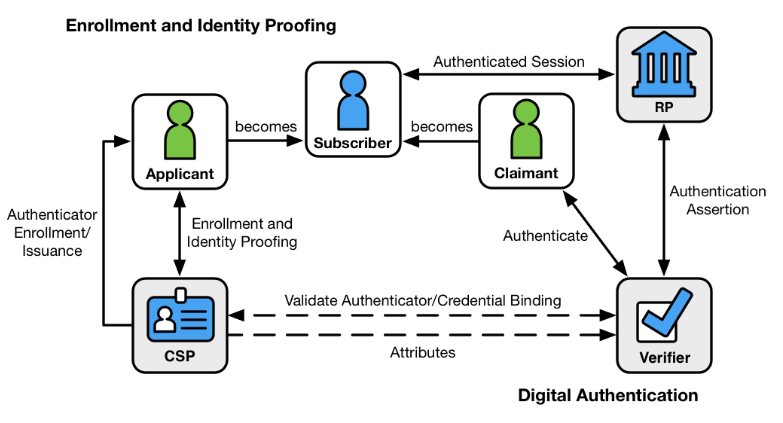
\includegraphics[width=0.7\textwidth]{DAM.png}
	\caption{NIST SP800.63B digital authentication model}
	\label{DAM}
\end{figure}

\subsection{Custom login con with standalone implementation}
In this case the verifier and the CSP are the embedded in the API server, that is the relying party.
\subsubsection*{Direct use of tokens and sessions}
%Pros and cons
\begin{itemize}
	\item \textbf{Pros:}
	\begin{itemize}
		\item greater implementation flexibility;
		\item less dependence on external services (hosting platform only).
	\end{itemize}
	\item \textbf{Cons:}
	\begin{itemize}
		\item double implementation required for direct login and social login (also required for internal members);
		\item authentication and related security systems not at the level of ad-hoc professional platforms.
	\end{itemize}
\end{itemize}

\subsection*{Use of external libraries (es. Passport)}
%Pros and cons
\begin{itemize}
	\item \textbf{Pros:}
	\begin{itemize}
		\item less dependence on external services (hosting platform only);
		\item predisposition to social login (Google, LinkedIn).
	\end{itemize}
	\item \textbf{Cons:}
	\begin{itemize}
		\item improved architecture compared to direct use, but with security features still delegated to the developer (e.g. rate limit).
	\end{itemize}
\end{itemize}

\subsection{Social login Provider}
In this case the verifier and the CSP are external to the API server: their functionalities are provided by the social provider of choice (e.g. Google, LinkedIn).

%Pros and cons
\begin{itemize}
	\item \textbf{Pros:}
	\begin{itemize}
		\item authentication and security measures delegated to external services;
		\item authentication and related professional security systems;
		\item Delegated Identity Management (authentication data management and security issues are delegated).
	\end{itemize}
	\item \textbf{Cons:}
	\begin{itemize}
		\item need to implement more services to guarantee more authentication alternatives to users;
		\item impossibility of simple registration to the WebApp, users are bound to have an account of at least one of the services offered. This does not arise for HKN members, given the associative email, but it is potentially limiting for applicants.
	\end{itemize}
\end{itemize}

\subsection{Third party custom service (Auth0, Amazon Cognito, Okta)}
In this case the verifier is the third party authentication server while the CSP is that same entity in case of traditional login with reusable password, or the social provider when that feature is used.
%Pros and cons
\begin{itemize}
	\item \textbf{Pros:}
	\begin{itemize}
		\item authentication and security measures delegated to external services;
		\item authentication and related professional security systems;
		\item Delegated Identity Management (authentication data management and security issues are delegated);
		\item possibility of access via social login provider (Google).
	\end{itemize}
	\item \textbf{Cons:}
	\begin{itemize}
		\item possible, but limited customization possibilities;
		\item limitation of 7000 active users / month with the free plan;
		\item double dependency to external platforms (hosting platform and authentication service).
	\end{itemize}
\end{itemize}

\subsection{Our choice}
Basing on the motivations above, our choice is to use a third party custom service. For this purpose, we compared the two major solutions available on the market: Auth0 and Amazon Cognito.

Amazon Cognito and Auth0 are both authentication tools. They are most commonly used by developers to implement on mobile or web applications being built. 
Amazon Cognito is used across company sizes, particularly companies that already live in the Amazon tech ecosystem. It’s ideal for 1st-party applications built for in-house use. In contrast, Auth0 is most commonly used by smaller organizations or teams, particularly those that can make use of the tool’s free version. Auth0 excels at helping these teams implement and manage authentication across services or apps, or across multiple clients. 
\subsection*{Features}
Amazon Cognito and Auth0 focus on serving distinct audiences, and they emphasize different feature strengths accordingly. 
Amazon Cognito stands out for its use in Amazon environments, although it is still a strong option beyond Amazon apps. It’s also ideal for managing authentication across multiple internally-facing or used tools. \textbf{This means that Cognito is often the first choice for internal applications built on Amazon infrastructure.} It also provides a range of sign-on capabilities, including integrating with 3rd-party ID providers like Microsoft Active Directory. 
\textbf{Auth0 provides stronger support and features for smaller-scale teams and companies.} For instance, it provides excellent documentation, as well as a mix of prebuilt and customizable authentication methods. \textbf{Auth0 is also much cheaper to initially get off the ground, with a robust free version that can suffice for very small use cases.} It also provides a more user-friendly administrative interface relative to other authentication providers. 
\subsection*{Limitations}
Amazon Cognito and Auth0 also each have some limitations worth considering. 
\textbf{Amazon Cognito is less accessible to smaller or less advanced developers.} While it offers more advanced features, those capabilities lack sufficient documentation for some reviewers, which can create a \textbf{longer and more intensive learning curve}, even among skilled developers. It also makes customization more complex to develop and implement than comparable authentication products.
On the other hand, Auth0 is less scalable for midsize and large companies. Its customizability at higher levels is much more limited, both in terms of functionality and branding or design. Auth0’s pricing structure also makes it less ideal for companies as they scale up. Companies should ensure that the initial pricing structure is efficient for their needs, and make sure that they don’t scale out of cost-efficiency as they grow.  

\subsection{Single Sign-On with Auth0 and authentication flow}
Single Sign-On (SSO) authentication is now required more than ever. Nowadays, almost every website requires some form of authentication to access its features and content. With the number of websites and services rising, a centralized login system has become a necessity.
Sooner or later web development teams face one problem: you have developed an application at domain X and now you want your new deployment at domain Y to use the same login information as the other domain. In fact, you want more: you want users who are already logged-in at domain X to be already logged-in at domain Y. This is what SSO is all about.
Whenever users go to a domain that requires authentication, they are redirected to the authentication domain. As users are already logged-in at that domain, they can be immediately redirected to the original domain with the necessary authentication token.
Auth0 Single Sign-On (SSO) solution works as a bridge between different SSO frameworks: Figure \ref{fig:SSOn} describes the mechanism. For more details, see the official article \href{https://auth0.com/blog/what-is-and-how-does-single-sign-on-work/}{\textit{What Is and How Does Single Sign-On Authentication Work?}}

\begin{figure}[ht]
	\centering
	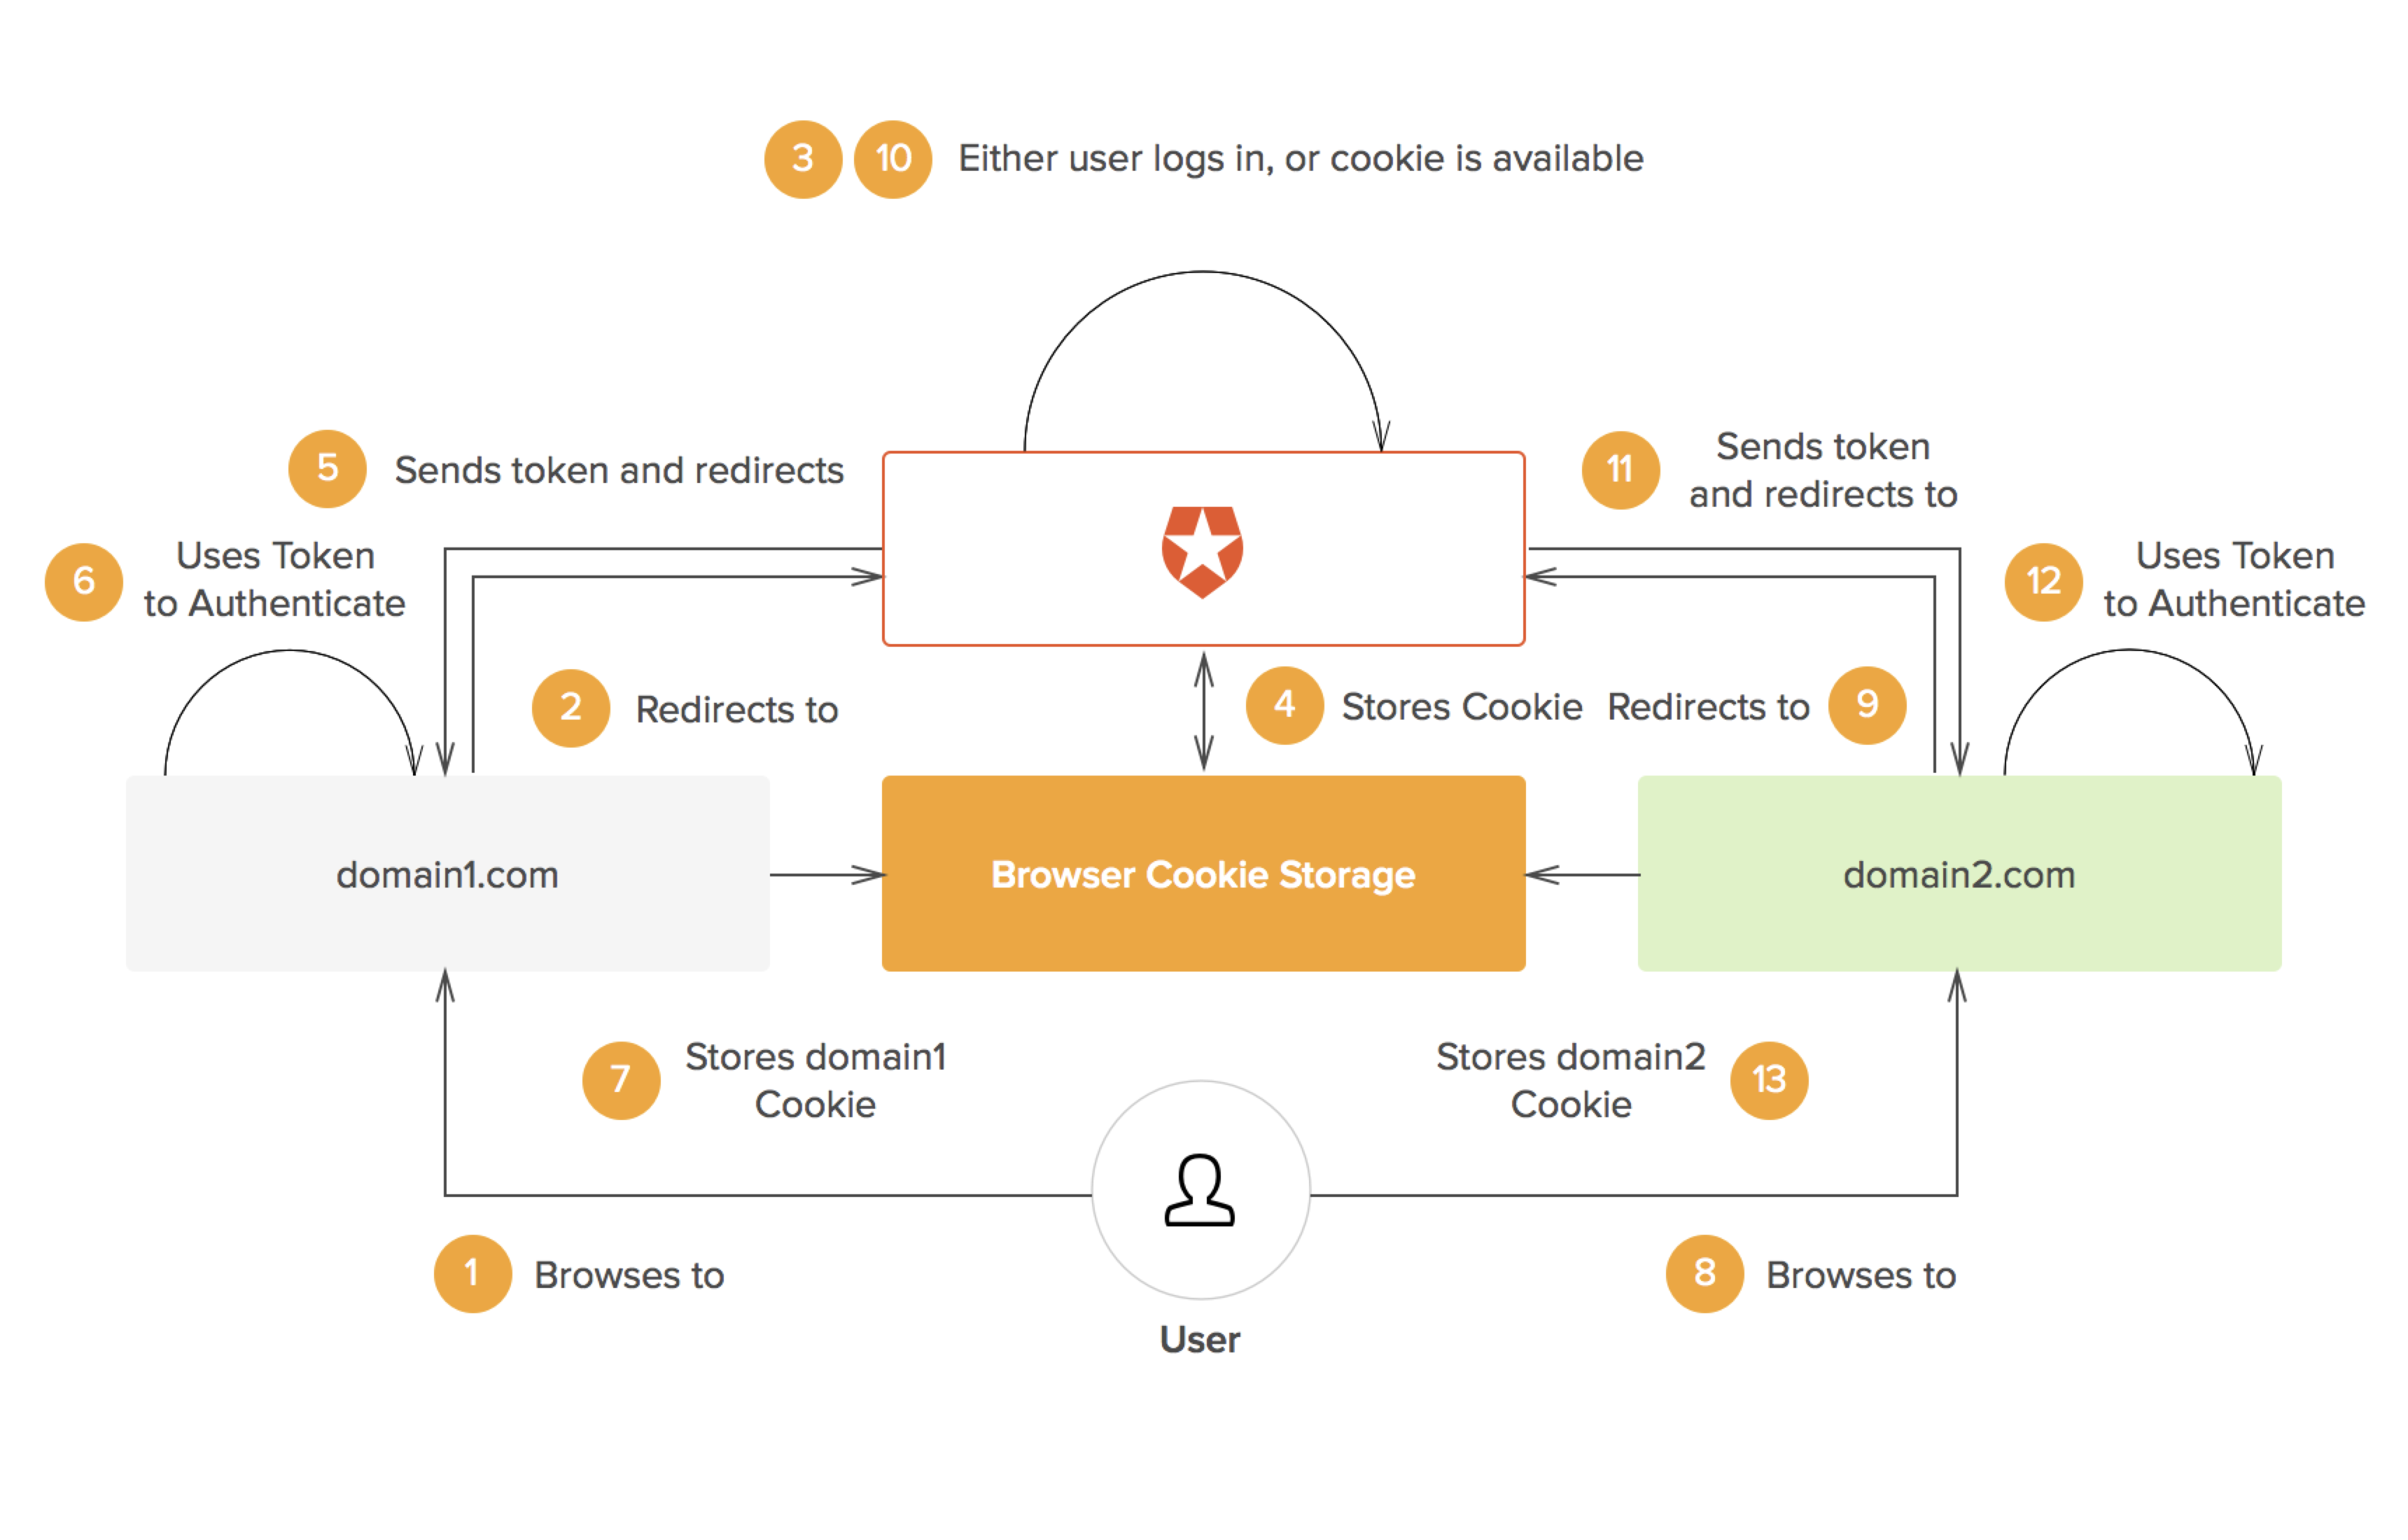
\includegraphics[width=0.9\textwidth]{auth0.png}
	
	\caption{Auth0 Single Sign-On (SSO) solution}
	\label{fig:SSOn}
\end{figure}

\subsection*{What happens when an application is composed by a React front-end and an API server}
When, like in this project, the application is a \textit{Single-Page Application} communicating with an API server, the authentication system is different from the classical one in which the server communicates with the verifier to authenticate the user. With machine-to-machine (M2M) applications, such as CLIs, daemons, or services running on your back-end, the system authenticates and authorizes the app rather than a user. For this scenario, typical authentication schemes like username + password or social logins don't make sense. Instead, M2M apps use the Client Credentials Flow (defined in OAuth 2.0 RFC 6749, section 4.4), in which they pass along their Client ID and Client Secret to authenticate themselves and get a token. Figure \ref{fig:ClientCredentialFlowAuth0} shows the Client Credentials Flow in Auth0: for more details see \href{https://auth0.com/docs/flows/client-credentials-flow}{\textit{Client Credentials Flow}}. An important detail to point out is that the API server will contact Auth0 to be able to verify the authenticity and integrity of the token received by the front-end app: for more details see \href{https://auth0.com/docs/tokens/json-web-tokens/validate-json-web-tokens}{\textit{Validate JSON Web Tokens}}.

\begin{figure}[ht]
	\centering
	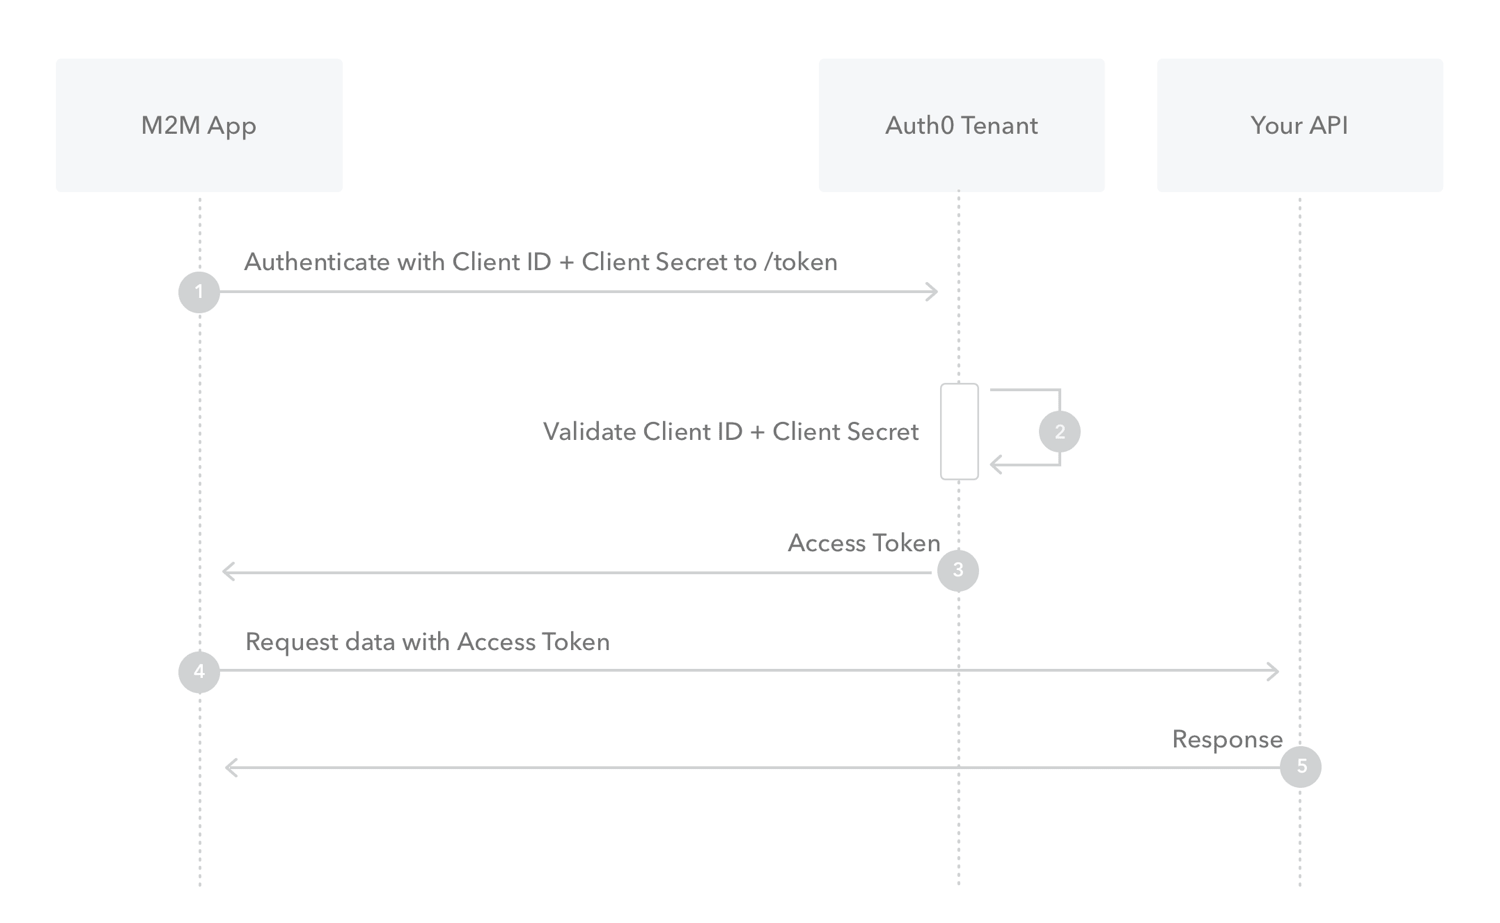
\includegraphics[width=0.9\textwidth]{auth-sequence-client-credentials.png}
	
	\caption{Client Credentials Flow in Auth0}
	\label{fig:ClientCredentialFlowAuth0}
\end{figure}

\subsection*{What does an Auth0 JWT contain?}
JSON web tokens (JWTs) claims are pieces of information asserted about a subject. In a JWT, a claim appears as a name/value pair where the name is always a string and the value can be any JSON value. It is possible to read more about this subject on \href{https://auth0.com/docs/tokens/json-web-tokens/json-web-token-claims}{\textit{JSON Web Token Claims}} webpage.

As per default, a token that will be received by the front-end application will contain at least the following claims:
\begin{lstlisting}[language=json]
{
"name": "John Doe",
"nickname": "john.doe",
"picture": "https://myawesomeavatar.com/avatar.png",
"updated_at": "2017-03-30T15:13:40.474Z",
"email": "john.doe@test.com",
"email_verified": false,
"sub": "auth0|USER-ID",
}
\end{lstlisting}
Among these, three claims are important for our purposes:
\begin{itemize}
	\item \texttt{email}: is the email used to sign up or log in. During registration phase, its value can be taken as default value. Please note that the is no constraint for a user on changing its email address: in this case the new address will be used when its necessary to contact the user, but the authentication will still use the address used during sign up;
	\item \texttt{email\_verified}: indicates whether the user has verified the email address provided during sign up. This value van be used by the client and the API server as an additional check that the user is a real one, for example forbidding the proceed with registration if the value is \texttt{false};
	\item \texttt{sub}: it is used as user identification inside our system.
\end{itemize}

\subsection{How this impacts on our system}
When logging in, the system should understand if the logged user is a member or an applicant. This somehow imposes this information to be required during logging in phase, and then confirmed by looking into the database. Because the login form is not entirely on our control, this can be non trivial.
After having considered several possibilities, the easiest and fastest one is to impose the following rules on user registration:
\begin{itemize}
	\item Member users can sign up only by using their official HKN email address, either using the "sign up with Google" or by inserting the email address. Any other email address associated with the registration of a member will lead to an error;
	\item Applicants can use whatever supported method. A registration of a member with an HKN email address will lead to an error;
	\item Since now it is possible that the same person is associated with two different account that have associated different email addresses, so two different entries in the person table, the uniqueness constraint on the \texttt{phone\_no} attribute must be changed: now two different members or two different applicants cannot share the same \texttt{phone\_no}.
\end{itemize}
In such a way, the system is able to determine if a user is a member or an applicant by looking at the email address only, that is contained inside the json web token (JWT) exchanged with Auth0.
%File: specifications.tex
%Data creazione: 31/12/2020
%Data ultima modifica: 31/12/2020

\chapter{Technical specifications}

\section{Information model}
\subsection{Enums}

\subsubsection{ApplicationState}
\begin{itemize}
    \item New: "new"
    \item Accepted: "accepted"
    \item Rejected: "rejected"
    \item Confirmed: "confirmed"
    \item Finalized: "finalized"
    \item RefusedByApplicant: "refused\_by\_applicant"
\end{itemize}


\subsubsection{ApplicationType}
\begin{itemize}
    \item BSC: "bsc"
    \item MSC: "msc"
    \item PHD: "phd"
\end{itemize}


\subsubsection{LangLevel}
\begin{itemize}
    \item B2: "B2"
    \item C1: "C1"
    \item C2: "C2"
    \item NativeSpeaker: "native\_speaker"
\end{itemize}

\subsection{DTOs}


\section{Database schema}

\section{RESTful APIs}
% GET /applications

\subsection{\texttt{\textcolor{blue}{GET} /v1/applications}}

Returns a list of all applications. 
If any query parameters are provided, applications are filtered accordingly. 
The response includes only applications and their details that are authorized for the requesting user. 

\subsubsection{Query Parameters}
\begin{itemize}
    \item \textbf{submittedFrom} [Date] (optional): Start date of the time period for filtering applications.
    \item \textbf{submittedUntil} [Date] (optional) : End date of the time period for filtering applications.
    \item \textbf{state} [ApplicationState] (optional): Retrieve only applications with this state. 
\end{itemize}

\subsubsection{Path Variables}
None

\subsubsection{Request Body}
None

\subsubsection{Response Body}
Array of \textbf{ApplicationResponseDto} objects.

% GET /applications/:application_id

\subsection{\texttt{\textcolor{blue}{GET} /v1/applications/:application\_id }}

Returns the details of a specific application identified by its ID.

\subsubsection{Query Parameters}
None

\subsubsection{Path Variables}
\begin{itemize}
    \item \textbf{application\_id} [Integer]: The ID of the application to retrieve.
\end{itemize}

\subsubsection{Request Body}
None

\subsubsection{Response Body}
An \textbf{ApplicationResponseDto} object representing the application details.

% POST /applications

\subsection{\texttt{\textcolor{blue}{POST} /v1/applications}}

Submits a new application for the logged-in user. 
The newly created application state is set to \textbf{ApplicationState.New}.
% TODO: A new Interview is created and associated to the application.
The operation will fail if the applicant already has a pending application.

\subsubsection{Query Parameters}
None

\subsubsection{Path Variables}
None

\subsubsection{Request Body}
A \textbf{CreateApplicationDto} object.
The body of the request must be encoded as \textbf{multipart/form-data}.
The "cv" and the optional "grades" files must be uploaded respectively as two fields with name "cv" and "grades".

\subsubsection{Response Body}
The newly created \textbf{Application} object.

% PATCH /v1/applications/:application_id

\subsection{\texttt{\textcolor{blue}{PATCH} /v1/applications/:application\_id}}

Updates the details of an existing application identified by its ID. 
If the user is an applicant, they can only update the application state to \textbf{ApplicationState.RefusedByApplicant}.
Other registered users can update the application state and notes.

\subsubsection{Query Parameters}
None

\subsubsection{Path Variables}
\begin{itemize}
    \item \textbf{application\_id} [Integer]: The ID of the application to update.
\end{itemize}

\subsubsection{Request Body}
A \textbf{UpdateApplicationDto} object.

\subsubsection{Response Body}
An \textbf{ApplicationResponseDto} object representing the updated application.

\section{Software architecture}

\section{Integration with Google RESTful APIs}

%File: testing.tex
%Data creazione: 31/12/2020
%Data ultima modifica: 31/12/2020

\chapter{Testing}
\section{Techniques and tools}
\section{Test coverage}


\appendix
\include{appendix/GNUFreeDocumentationLicense}

%%%%%%%%%%%%%%%%%%%%%%%%%%%%%%%%%%%%%%%%%%%%%%%%%%%%%%%%%%%%%%%%%%%%%%%%%%%%%%%%%%%%%%%%%


\end{document}